\documentclass[12pt]{article}

% Ustawienia strony
\usepackage{lipsum}
\usepackage[margin=1.5cm]{geometry}
\usepackage{graphicx}
\usepackage{enumitem}
\usepackage{siunitx}
\usepackage{amsmath}
\usepackage{cancel}
\usepackage{makecell}
\usepackage{mathtools}
\usepackage{floatrow}
\usepackage{caption}
\usepackage[T1]{fontenc}
\usepackage{fancyvrb}
\usepackage[ngerman]{babel} %Deutsche Sprachunterstützung
\usepackage{subcaption}
\usepackage{graphicx}
\usepackage{blindtext}
\usepackage{hyperref}
\usepackage[dvipsnames]{xcolor}

\hypersetup{
	colorlinks=true,
	linkcolor=blue,
	filecolor=magenta,      
	urlcolor=cyan,
	pdfpagemode=FullScreen,
}

\urlstyle{same}

\fvset{tabsize=4}
\setlist{leftmargin=15pt,labelindent=15pt}
\setlist[enumerate]{noitemsep,wide=0pt, leftmargin=*}
{\setlength{\parindent}{0pt}

% Ustawienia stopki
\usepackage{lastpage}
\usepackage{fancyhdr}
\pagestyle{fancy}
\fancyhf{} % sets both header and footer to nothing
\renewcommand{\headrulewidth}{0pt}
\cfoot{\thepage\ z \pageref*{LastPage}}

\begin{document}

\section*{Podstawowe dane}
\begin{figure}[htp]
	\begin{minipage}[t]{0.3\textwidth}
		\textbf{Imie i nazwisko} \\
		\textbf{Data} \\
		\textbf{Tytuł} \\
		\textbf{Numer ćwiczenia}
	\end{minipage}%
	\begin{minipage}[t]{0.6\textwidth}
		Robert Mesek \\
		30.11.2023 \\
		Algorytmy geometryczne \\
		3
	\end{minipage}%
\end{figure}

\section*{Dane techniczne}
\begin{figure}[htp]
	\begin{minipage}[t]{0.3\textwidth}
		\textbf{Procesor} \\
		\textbf{Język} \\
		\textbf{Biblioteki} \\
		\textbf{System operacyjny} \\
		\textbf{Środowisko}

	\end{minipage}%
	\begin{minipage}[t]{0.6\textwidth}
		Intel i7-1165G7 x86\_64 \\
		Python 3.11.5 \\
		NumPy 1.26.0, Pandas 2.1.1, Matplotlib 3.8.0 \\
		WSL Ubuntu 22.04 (MS Windows 10 22H2) \\
		conda 23.5.2
	\end{minipage}%
\end{figure}

\subsection*{Cel ćwiczenia}
\begin{figure}[htp]
	\begin{minipage}[t]{0.5\textwidth}
		\vspace{1em}
		
		Celem ćwiczenia jest:
		
		- sprawdzanie $y$-monotoniczności
		
		- podział wierzchołków na kategorie
		
		- triangulacja wielokąta monotonicznego
	\end{minipage}%
	\hfill
	\begin{minipage}[t]{0.5\textwidth}
		\centering
		\vspace{0pt}
		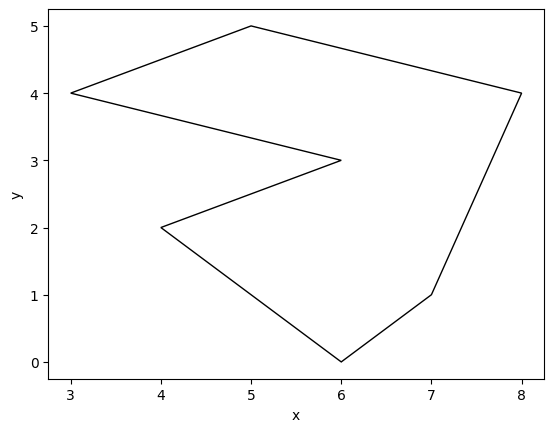
\includegraphics[width=1\linewidth]{images/przyklad.png}
		
		\verb|przyklad|: wielokąt y-monotoniczny
	\end{minipage}%
	\hspace*{\fill}
\end{figure}

\subsection*{Zastosowania triangulacji} 
Triangulacja wielokątów w informatyce znajduje zastosowanie w grafice komputerowej, w algorytmach geometrii obliczeniowej do rozwiązywania problemów związanych z przetwarzaniem i analizą danych przestrzennych oraz analizowania sieci.

\newpage

\subsection*{Wielokąty}
\par

\begin{figure}[H]
	\centering
	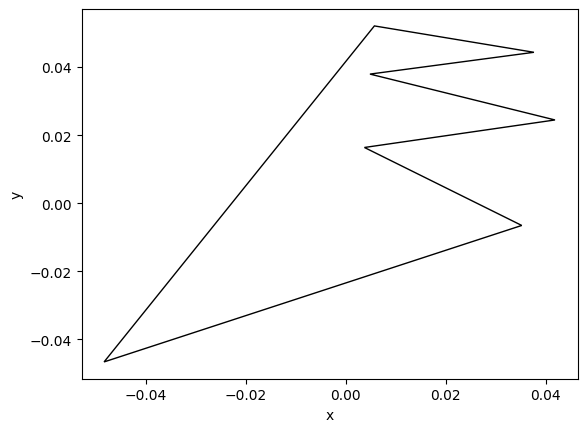
\includegraphics[width=0.7\linewidth]{images/polygon-a.png}
	
	\verb|polygon_a|
\end{figure}


\begin{figure}[H]
	\centering
	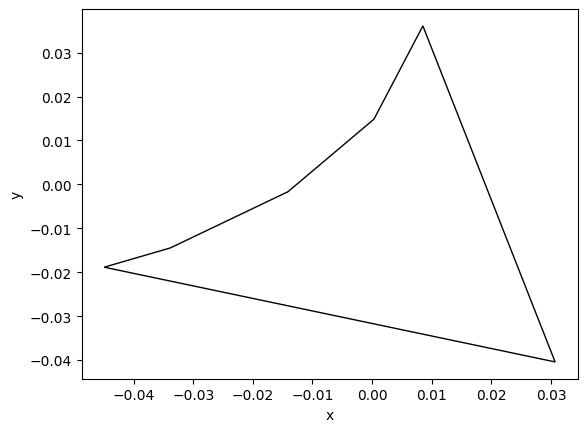
\includegraphics[width=0.7\linewidth]{images/polygon-b.png}
	
	\verb|polygon_b|
\end{figure}

\newpage

\par

\begin{figure}[H]
	\centering
	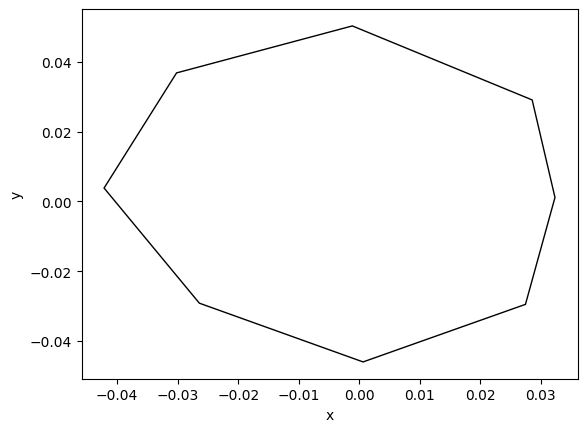
\includegraphics[width=0.7\linewidth]{images/polygon-c.png}
	
	\verb|polygon_c|
\end{figure}

\par

\begin{figure}[H]
	\centering
	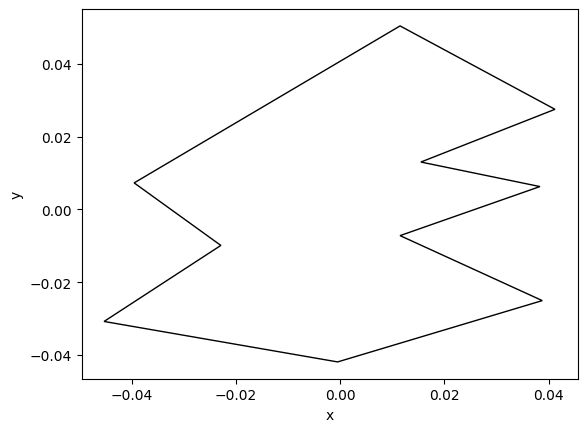
\includegraphics[width=0.7\linewidth]{images/polygon-d.png}
	
	\verb|polygon_d|
\end{figure}

\newpage

\section*{Funkcje pomocnicze}

\par Reprezentuje punkt
\begin{Verbatim}
class Point:
	EPSILON = 10**-24
	
	def __init__(self, x, y, id=None, type=None):
		self.x = x
		self.y = y
		self.id = id
	
	def __repr__(self):
		return f"{self.id}. ({self.x}, {self.y})"
	
	def distance(self, other):
		return ((other.x - self.x) ** 2 + (other.y - self.y) ** 2) ** 0.5
	
	def as_tuple(self):
		return (self.x, self.y)
	
	def __hash__(self) -> int:
		return hash((self.x, self.y, self.id))
	
	def __eq__(self, other: object) -> bool:
		if not isinstance(other, Point):
			return NotImplemented
		return self.distance(other) < self.EPSILON
	
	def __gt__(self, other: object) -> bool:
		if not isinstance(other, Point):
			return NotImplemented
		if abs(self.x - other.x) < self.EPSILON:
			return self.y > other.y
		return self.x > other.x
\end{Verbatim}

\mbox{}
\par Konwertuje listę krotek na listę punktów
\begin{Verbatim}
def create_points(Q: list[tuple]):
	points = []
	for i, (x, y) in enumerate(Q):
		points.append(Point(x, y, i))
	return points
\end{Verbatim}

\newpage

\mbox{}
\par Oblicza wyznacznik macierzy, potrzebny do określenia orientacji punktu względem prostej
\begin{Verbatim}
def det(a: Point, b: Point, c: Point):
	"""
	Orientacja punktu "c" względem prostej "a b" obliczając wyznacznik macierzy 2x2
	:param a: pierwszey punkt tworzący naszą prostą
	:param b: drugi punkt tworzący naszą prostą
	:param c: punkt, którego położenie względem prostej chcemy znaleźć
	:return: wartość wyznacznika macierzy
	(> 0) => Counterclockwise
	(== 0) => Collinear
	(< 0) => Clockwise
	"""
	return (a.x - c.x) * (b.y - c.y) - (a.y - c.y) * (b.x - c.x)
\end{Verbatim}

\mbox{}
\par Klasyfikuje punkt
\begin{Verbatim}
def classify(a: Point, b: Point, c: Point, eps=Point.EPSILON):
	"""
	:return: klasyfikacja punktu
	starting = 0
	closing = 1
	connective = 2
	separative = 3
	correct = 4
	"""
	# starting or separative or correct
	if a.y < b.y and c.y < b.y:
		# starting = 0
		if det(a, b, c) > eps:
			return 0
		# separative = 3
		elif det(a, b, c) < -eps:
			return 3
	# closing or connective or correct
	elif a.y > b.y and c.y > b.y:
		# closing = 1
		if det(a, b, c) > eps:
			return 1
		# connective = 2
		elif det(a, b, c) < -eps:
			return 2
	# correct = 4
	else:
	return 4
\end{Verbatim}

\newpage

\section*{Czy wielokąt jest y-monotoniczny?}
\par 
Wielokąt jest monotoniczny, gdy jego wierzchołki mogą być ułożone w taki sposób, że jedna z jego współrzędnych (na przykład współrzędna $x$ lub $y$, w zależności od układu współrzędnych) zawsze rośnie lub maleje wzdłuż kolejnych wierzchołków. Innymi słowy, dla każdej pary wierzchołków wielokąta (oprócz wierzchołka startowego i końcowego), jeden z punktów ma większą (lub mniejszą) wartość danej współrzędnej niż drugi punkt.
\newline\newline
W praktyce, wielokąt monotoniczny może być łatwiej sortowany lub przetwarzany w pewnych algorytmach geometrycznych, ponieważ istnieje pewna kolejność, w jakiej wierzchołki pojawiają się wzdłuż danej osi (np. osi $x$ lub $y$). Monotoniczność może ułatwić znajdowanie przecięć linii w takim wielokącie lub wykonywanie innych operacji geometrycznych. W tym zadaniu interesuje nas monotoniczność wielokąta wzdłuż osi $y$.


\subsection*{Funkcja sprawdzająca czy wielokąt jest y-monotoniczny}
\begin{Verbatim}
def is_y_monotonic(polygon):
	"""
	Funkcja określa czy podana figura jest y-monotoniczna.
	:param polygon: tablica krotek punktów na płaszczyźnie euklidesowej podanych 
	przeciwnie do ruchu wskazówek zegara - nasz wielokąt
	:return: wartość bool - true, jeśli wielokąt jest monotoniczny i false jeśli nie jest
	"""
	points = create_points(polygon)
	
	for i in range(len(points) - 1):
		# connective or separative
		if classify(points[i - 1], points[i], points[i + 1]) in (2, 3):
			return False
	# connective or separative
	if classify(points[-2], points[-1], points[0]) in (2, 3):
		return False
	return True
\end{Verbatim}

\newpage

\section*{Podział wierzchołków na kategorie}
\par 
Wierzchołki naszego wielokąta możemy podzielić na parę kategorii:

- początkowe, gdy obaj jego sąsiedzi leżą poniżej i kąt wewnętrzny ma mniej niż 180 stopni. To wierzchołki, w których zaczyna się monotoniczny spadek

- końcowe, gdy obaj jego sąsiedzi leżą powyżej i kąt wewnętrzny ma mniej niż 180 stopni. To wierzchołki, w których monotoniczność wielokąta się zmienia, czyli na przykład zaczyna się monotoniczny wzrost, jeśli wcześniej był spadek, lub na odwrót.
\newline\newline
Wierzchołki startowe i końcowe są ważne w kontekście algorytmów przetwarzania wielokątów monotonicznych, takich jak algorytmy dziel i zwyciężaj oraz triangulacji.

- dzielący, gdy obaj jego sąsiedzi leżą poniżej i kąt wewnętrzny ma więcej niż 180 stopni. To wierzchołki, które wyznaczają przekątne (linie łączące), tworzące trójkąty podczas triangulacji.

- łączący, gdy obaj jego sąsiedzi leżą powyżej i kąt wewnętrzny ma więcej niż 180 stopni. To wierzchołki, które są połączone liniami (przekątnymi) wewnątrz wielokąta, tworząc trójkąty.
\newline\newline
Wierzchołki łączące i dzielące odgrywają kluczową rolę w procesie triangulacji wielokątów, pozwalając na podział figury na trójkąty w sposób bezkolizyjny.

- prawidłowy, pozostałe przypadki, jeden sąsiad powyżej, drugi poniżej

\section*{Znaczenie kolorów}
\begin{itemize}
	\item Początkowy - \color{ForestGreen}kolor zielony\color{black}
	\item Końcowy - \color{red}kolor czerwony\color{black}
	\item Łączący - \color{blue}kolor niebieski\color{black}
	\item Dzielący - \color{cyan}kolor cyjan\color{black}
	\item Prawidłowy - \color{Sepia}kolor brązowy\color{black}
\end{itemize}
\par 

\newpage

\section*{Funkcja przypisująca kolory wierzchołkom}
\begin{Verbatim}
def color_vertex(polygon):
	"""
	Funkcja dzieli wierzchołki na kategorie i przypisuje wierzchołkom odpowiednie numery: 
	0 - początkowy, 1 - końcowy, 2 - łączący, 3 - dzielący, 4 - prawdiłowy
	:param polygon: tablica krotek punktów na płaszczyźnie euklidesowej podanych 
	przeciwnie do ruchu wskazówek zegara - nasz wielokąt
	:return: tablica o długości n, gdzie n = len(polygon), zawierająca cyfry z przedziału 
	0 - 4, gdzie T[i] odpowiada kategorii i-tego wierzchołka.
	"""
	points = create_points(polygon)
	colors = []
	
	# all points excep first and last
	for i in range(0, len(points) - 1):
		colors.append(classify(points[i - 1], points[i], points[i + 1]))
	# last point
	colors.append(classify(points[-2], points[-1], points[0]))
	
	return colors
\end{Verbatim}

\par
\begin{figure}[H]
	\centering
	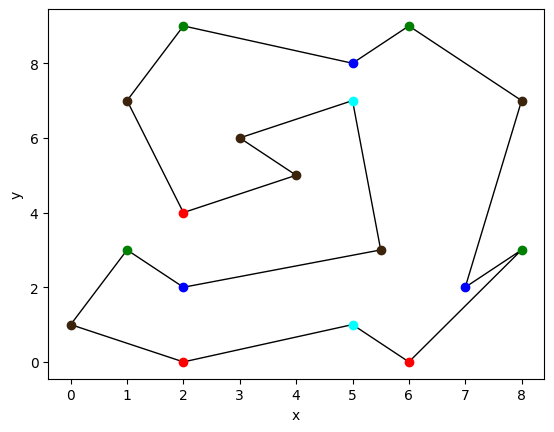
\includegraphics[width=0.7\linewidth]{images/przyklad-color.png}
	
	\verb|przyklad_color|: Podgląd wyniku funkcji \verb|color_vertex()|
\end{figure}

\newpage

\section*{Wyniki kolorowania dla naszych wielokątów}

\par

\begin{figure}[H]
	\centering
	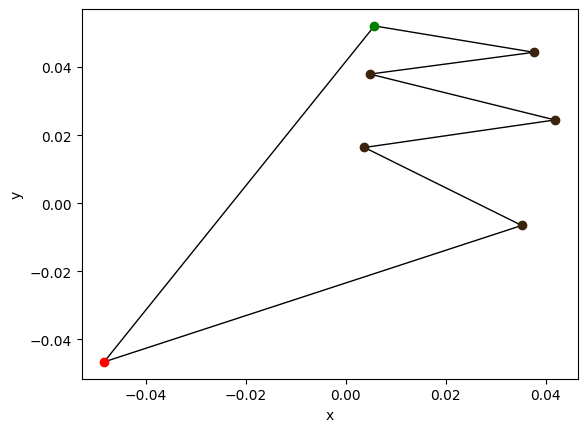
\includegraphics[width=0.7\linewidth]{images/color-a.png}
	
	\verb|polygon_a|
\end{figure}


\begin{figure}[H]
	\centering
	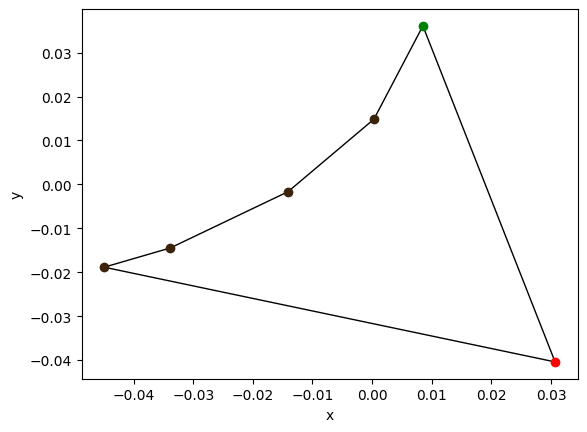
\includegraphics[width=0.7\linewidth]{images/color-b.png}
	
	\verb|polygon_b|
\end{figure}

\newpage

\par

\begin{figure}[H]
	\centering
	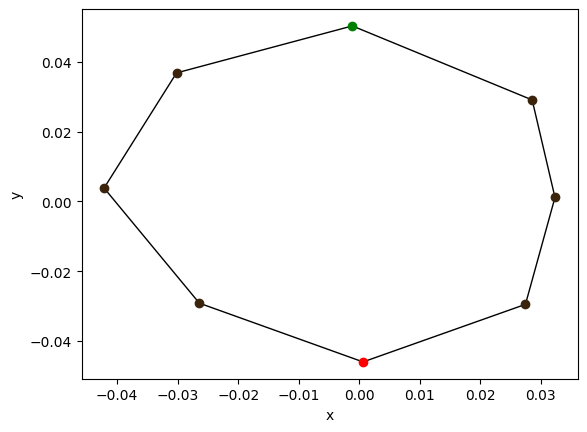
\includegraphics[width=0.7\linewidth]{images/color-c.png}
	
	\verb|polygon_c|
\end{figure}

\par

\begin{figure}[H]
	\centering
	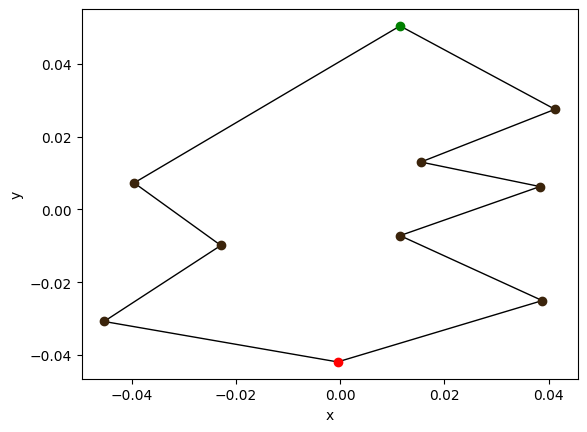
\includegraphics[width=0.7\linewidth]{images/color-d.png}
	
	\verb|polygon_d|
\end{figure}

\paragraph{Wnioski:}
\mbox{}\newline
Analizując wyniki, widzimy że wielokąty y-monotoniczne (wymaganie dla triangulacji naszym algorytmem) składają się wyłącznie z punktu początkowego, końcowego oraz wierzchołków prawidłowych.

\newpage

\section*{Triangulacja wielokąta monotonicznego}
\begin{figure}[htp]
	\begin{minipage}[t]{0.5\textwidth}
		\vspace{1em}
		
		Triangulacja wielokąta monotonicznego to proces podziału wielokąta monotonicznego na trójkąty poprzez dodawanie przekątnych (linii łączących wierzchołki), które nie przecinają się wewnętrznie.
	\end{minipage}%
	\hfill
	\begin{minipage}[t]{0.5\textwidth}
		\centering
		\vspace{0pt}
		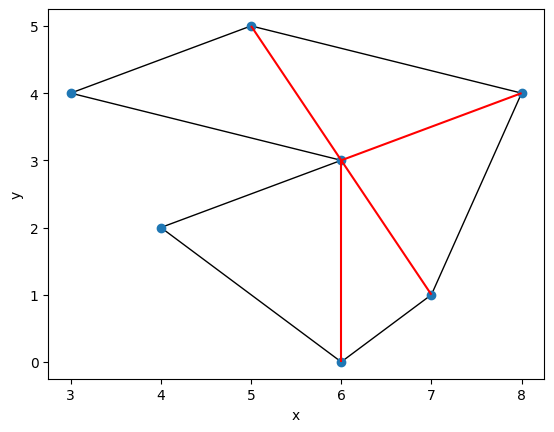
\includegraphics[width=1\linewidth]{images/przyklad-tri.png}
		
		\verb|przyklad_tri|: wielokąt podzielony na trójkąty
	\end{minipage}%
	\hspace*{\fill}
\end{figure}

\subsection*{Działanie implementowanego algorytmu (z wykładu)}
\begin{itemize}
	\item Określamy lewy i prawy łańcuch wielokąta względem kierunku monotoniczności
	\item Porządkujemy wierzchołki wzdłuż kierunku monotoniczności
	\item Wkładamy dwa pierwsze wierzchołki na stos.
	\item Jeśli kolejny wierzchołek należy do innego łańcucha niż wierzchołek stanowiący szczyt stosu,to możemy go połączyć ze wszystkimi wierzchołkami na stosie. Na stosie zostają dwa wierzchołki, które były „zamiatane” ostatnie.
	\item Jeśli kolejny wierzchołek należy do tego samego łańcucha co wierzchołek ze szczytu stosu, to analizujemy kolejne trójkąty, jakie tworzy dany wierzchołek z wierzchołkami zdejmowanymi ze stosu:
	\begin{itemize}
		\item Jeśli trójkąt należy do wielokąta, to dodajemy przekątną i usuwamy odpowiedni wierzchołek ze szczytu stosu
		\item w przeciwnym przypadku umieszczamy badane wierzchołki na stosie.
	\end{itemize}
\end{itemize}

\newpage

\subsection*{Funkcje pomocnicze dla triangulacji}
\mbox{}
\par Tworzy dwa \textbf{zbiory} (\verb|set()|): łańcuch punktów z lewej oraz prawej strony wielokąta
\begin{Verbatim}
def find_chains(points: list[Point]):
	right_chain = set()
	left_chain = set()
	starting = max(points, key=lambda x: x.y).id
	ending = min(points, key=lambda x: x.y).id
	i = ending
	while i != starting:
		right_chain.add(points[i])
		i = (i + 1) % len(points)
	while i != ending:
		left_chain.add(points[i])
		i = (i + 1) % len(points)
	return left_chain, right_chain
\end{Verbatim}

\mbox{}
\par Sprawdza czy dwa punkty należą do tego samego łańcucha
\begin{Verbatim}
def check_same_chains(left_chain, right_chain, p1: Point, p2: Point):
	if (p1 in left_chain and p2 in left_chain) 
		or (p1 in right_chain and p2 in right_chain):
		return True
	return False
\end{Verbatim}

\mbox{}
\par Sprawdza czy sprawdzany trójkąt znajduje się wewnątrz wielokąta
\begin{Verbatim}
def triangle_in_polygon(chain, a: Point, b: Point, c: Point, epsilon=Point.EPSILON):
	if b in chain:
		return det(a, b, c) > epsilon
	else:
		return det(a, b, c) < -epsilon
\end{Verbatim}

\mbox{}
\par Sprawdza czy wierzchołki są sąsiadami
\begin{Verbatim}
def check_neighbours(points: list[Point], a: Point, b: Point):
	if abs(a.id - b.id) == 1 or abs(a.id - b.id) == len(points) - 1:
		return True
	return False
\end{Verbatim}

\newpage

\subsection*{Funkcja triangulacji}
\begin{Verbatim}
def triangulation(polygon):
	"""
	Funkcja dokonuje triangulacji wielokąta monotonicznego.
	:param polygon: tablica krotek punktów na płaszczyźnie euklidesowej 
	podanych przeciwnie do ruchu wskazówek zegara - nasz wielokąt
	:return: tablica krotek dodawanych po kolei przekątnych np: [(1,5),(2,3)], 
	oznacza, że triangulacja polega na dodaniu przekątnej pomiędzy wierzchołki 
	o indeksach 1 i 5 oraz 2 i 3
	"""
	if not is_y_monotonic(polygon):
		raise Exception("Not y-monotonic")
	points = create_points(polygon)
	
	left_chain, right_chain = find_chains(points)
	points.sort(key=lambda x: x.y, reverse=True)
	
	stack = [points[0], points[1]]
	diagonals = []
	for i in range(2, len(points)):
		if not check_same_chains(left_chain, right_chain, stack[-1], points[i]):
			while len(stack) > 0:
				p = stack.pop()
				if not check_neighbours(points, p, points[i]):
					diagonals.append((points[i].id, p.id))
			stack.append(points[i - 1])
			stack.append(points[i])
		else:
			p = stack.pop()
			while len(stack) > 0 
				and triangle_in_polygon(left_chain, stack[-1], p, points[i]):
				if not check_neighbours(points, stack[-1], points[i]):
					diagonals.append((points[i].id, stack[-1].id))
				p = stack.pop()
			stack.append(p)
			stack.append(points[i])
	
	return diagonals
\end{Verbatim}

\newpage

\section*{Wyniki triangulacji dla naszych wielokątów}

\par

\begin{figure}[H]
	\centering
	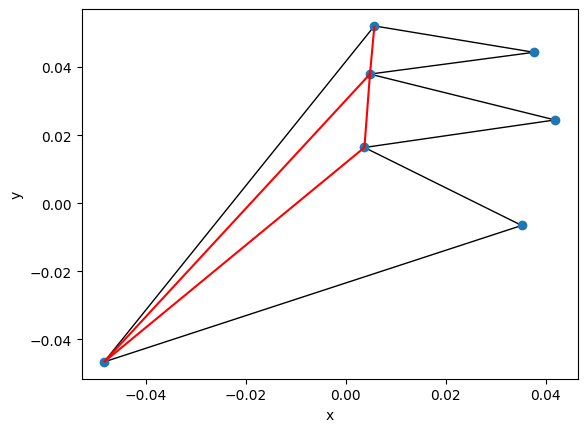
\includegraphics[width=0.7\linewidth]{images/tri-a.png}
	
	\verb|polygon_a|: Poruszamy się po prawym łańcuchu
\end{figure}


\begin{figure}[H]
	\centering
	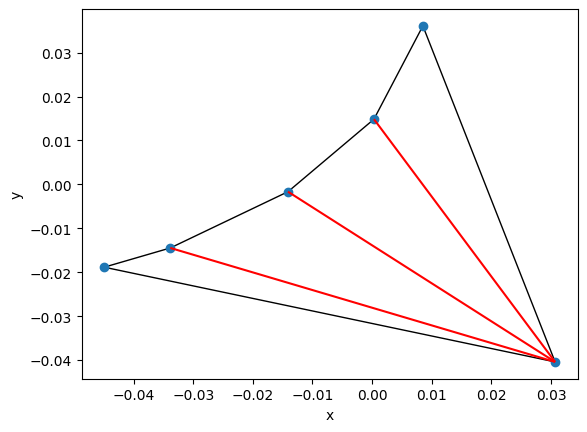
\includegraphics[width=0.7\linewidth]{images/tri-b.png}
	
	\verb|polygon_b|: Poruszamy się po lewym łańcuchu 
	
	i musimy wybierać trójkąty wewnątrz wielokąta
\end{figure}

\newpage

\par

\begin{figure}[H]
	\centering
	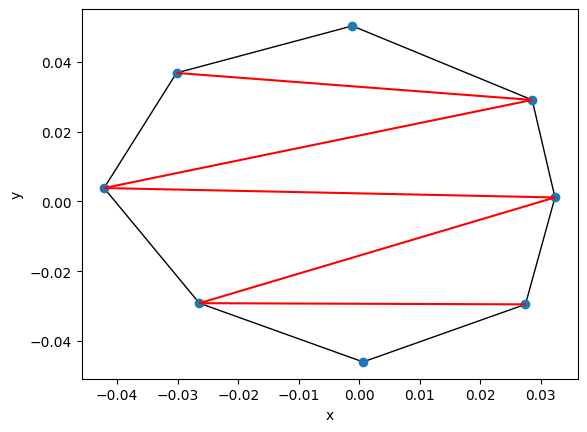
\includegraphics[width=0.7\linewidth]{images/tri-c.png}
	
	\verb|polygon_c|: Poruszamy się na przemian po łańcuchach
\end{figure}

\par

\begin{figure}[H]
	\centering
	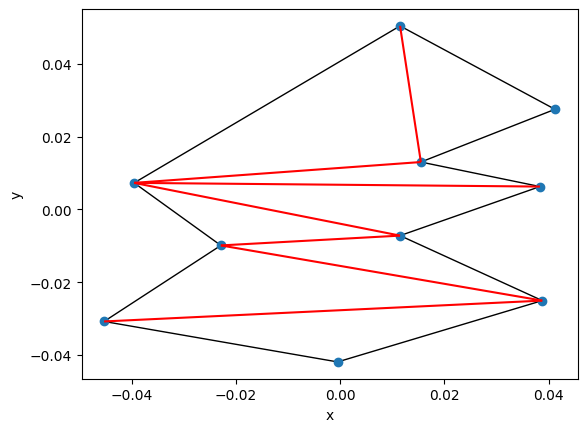
\includegraphics[width=0.7\linewidth]{images/tri-d.png}
	
	\verb|polygon_d|: "Listek" - połączenie różnych przypadków
\end{figure}

\paragraph{Wnioski:}
\mbox{}\newline
Analizując wyniki, widzimy że triangulacja dla naszych wielokątów y-monotonicznych została przeprowadzona poprawnie.

Dla takich małych zbiorów wierzchołków algorytm wykonywał się momentalnie: $<70$ ms.

\end{document}
